\documentclass[10pt,twocolumn,letterpaper]{article}
\usepackage[review]{cvpr}
\newif\ifexpandedpaper
\ifdefined\cvprcompact\expandedpaperfalse\else\expandedpapertrue\fi
% Additional packages; loaded before hyperref (see main.tex), as required by the CVPR 2027 author kit.
\usepackage{graphicx}
\usepackage{amsmath,amssymb}
\usepackage{booktabs}
\newcommand{\paperTitle}{High-Reach Candidate Search for Longitudinal Lung Lesion Matching}

\newcommand{\pp}{\,\mathrm{pp}}
% ---- added in revision ----
\usepackage{cuted}           % page-1 teaser strip
\usepackage{caption}
\usepackage{multirow}
\usepackage{algorithm}
\usepackage[noend]{algpseudocode}
\usepackage{xspace}
\newcommand{\TODO}[1]{\textbf{\color{red}[TODO: #1]}}
% \renewcommand{\TODO}[1]{}  % uncomment before submission
\DeclareMathOperator*{\argmax}{arg\,max}
\newcommand{\ours}{Diverse search\xspace}
\newcommand{\T}{\mathcal{T}}   % translation lattice
\newcommand{\Ss}{\mathcal{S}}  % retained (diversified) set
\usepackage{placeins}

\title{\paperTitle}
\author{Anonymous CVPR submission}
\hypersetup{pdftitle={\paperTitle}}

\begin{document}
\maketitle
\begin{abstract}
Finding the earlier location of a lung lesion in serial CT depends on which plausible locations survive the search. We order local translations by anatomical fit, retain spatially distinct hypotheses, and rank them with a fixed lesion scorer. On an independent staging cohort of 440 linked pulmonary metastases from 72 patients, this search places 289 earlier points within 3 mm of the reference, compared with 243 for a lesion-inclusive spline. The paired gain is 10.5 percentage points (95\% CI 3.6--17.6), alongside a 10.7-point gain (5.8--15.4) on 309 retrospective screening tracks. With the same 28-candidate budget, spatial diversification improves matching by 9.1 points in staging and 12.0 in screening compared with taking the top 28 translations by fit. The full diversified list retains 348 of 351 raw-reachable staging targets using about one-thirteenth of the candidate centers. On the same expanded strict candidate sets, the direct scorer selects 33 of 39 newly reachable staging targets, compared with 10 for SAM. Median local time on prepared staging crops is 0.194 s versus 3.617 s for the spline.

\end{abstract}

\begin{figure*}[!t]
\centering
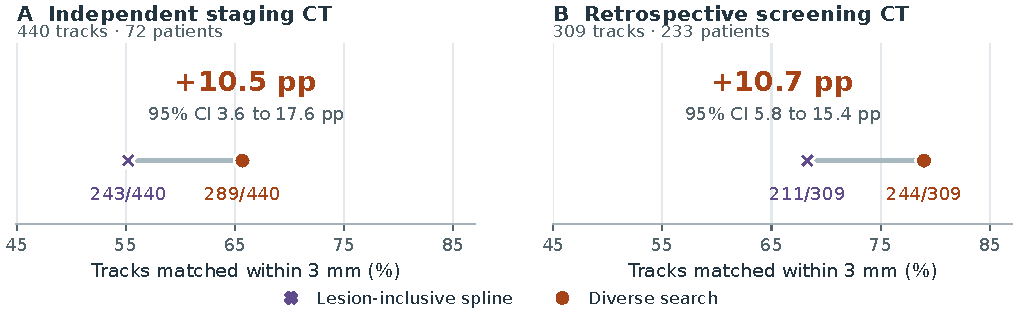
\includegraphics[width=\textwidth]{figures/cohort_transfer.pdf}
\caption{Diverse search improves 3 mm correspondence in two CT cohorts. The points show automatic hit rates on all allocated tracks. Each label gives the number of hits over the cohort total. The gain and interval above each pair come from a paired patient-cluster bootstrap. Both routes use the same current query, scan alignment and image support.}
\label{fig:transfer}
\end{figure*}

\section{Introduction}
Finding a lung lesion in an earlier CT links the same finding across visits for measurement of interval change~\cite{sofka2010,rafaelpalou2021}. We study the point-query setting, where a current lesion has already been identified and its approximate location is supplied. Chest alignment puts the two scans in a common frame. Breathing, positioning and changes in lesion appearance can leave several earlier locations plausible within that frame. Closely spaced shifts can also fill a shortlist with slight variations of the same alignment.

We propose a local search that uses anatomical agreement to order translations and reserves the final choice for a lesion scorer. In fit order, the search keeps a translation only if its mapped point is sufficiently far from previously retained points. At a fixed candidate count, the list covers more distinct locations. With the full list, every lattice point has a retained neighbor within the separation radius. Fit and witness residuals continue to inform the final score. The same current point, image support and scorer let us measure the effect of changing which points are considered.

On independent staging CT, the proposed search locates 289 of 440 linked pulmonary metastases within 3 mm, versus 243 for a lesion-inclusive deformable spline. It gains 10.5 percentage points and takes about one-nineteenth of the median local time on prepared staging crops. The same approach improves by 10.7 points in retrospective screening. At exactly 28 candidates per supported query, diversification alone adds 40 staging hits and 37 screening hits relative to a fit-ranked prefix (Fig.~\ref{fig:transfer}, Tab.~\ref{tab:contrasts}).

\ifexpandedpaperThe design separates two tasks that matter for interpreting a correspondence system. The first is to retain at least one usable location, which we measure as candidate \emph{reach}. The second is to select that location when other candidates are present. A sparse set makes the first task hard. A larger set gives the scorer more opportunities and more competitors. To isolate those effects we vary the cap at fixed physical support, compare fit-only and diversified prefixes of equal length, and score the same centers with two different functions. This gives a paired account of gains from additional reach and changes in choices on tracks already reachable.

This separation also makes compute a design variable. An exhaustive lattice provides a useful accuracy reference, while the full diversified search limits how many local descriptors need to be computed. We evaluate both and measure local matching separately from shared scan initialization. The staging data change the institution and clinical setting while preserving an independently linked 3D reference. The screening tracks provide a replication with a different lesion population and acquisition setting.
\fi

\section{Related work}
\paragraph{Local correspondence and registration.}
Location Registration and Recognition generates, refines and verifies local registration hypotheses for supplied nodule positions~\cite{sofka2010}. Deformable registration can estimate a continuous map that accommodates local motion~\cite{rueckert1999,ghazipour2021}. Studies of registration uncertainty distinguish image agreement from the reliability of a mapped location~\cite{eppenhof2018,luo2017}. Our study measures a complementary design choice in local hypothesis search. We isolate how the allocation of candidate centers affects target coverage and final selection under the same scan initialization. A lesion-inclusive spline supplies a continuous-registration comparison.

\paragraph{Learned lesion matching.}
Rafael-Palou \etal~\cite{rafaelpalou2021} use a learned representation to re-identify detected nodules. Deep Lesion Tracker and Transformer Lesion Tracker combine lesion appearance with anatomical context~\cite{cai2021,tang2022tlt}. Dense anatomical embeddings enable correspondence from a point query~\cite{yan2022sam,zhuang2026diffusion}. SAM offers a released point-query checkpoint and a dense similarity field. This lets us compare its selected point and cross its scorer with the same candidate sets used by our local matcher. The crossing varies candidate allocation while holding the scored positions, current query and input crops fixed for each budget.

\section{Fit-ordered diverse search}
\label{sec:method}

\begin{figure*}[!t]
\centering
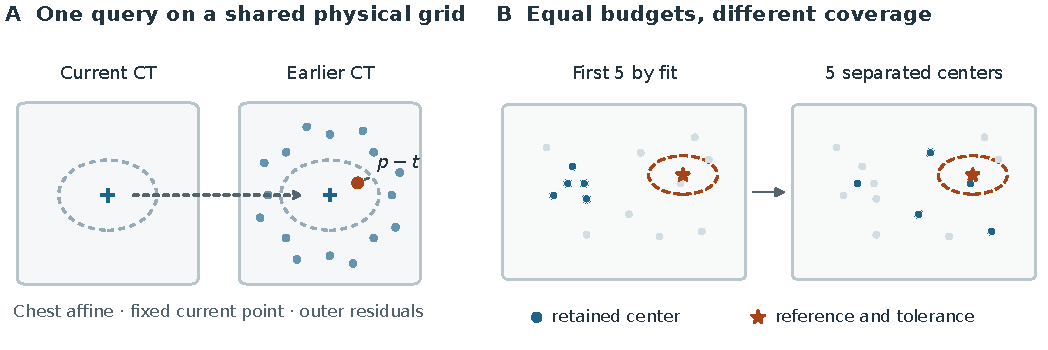
\includegraphics[width=\textwidth]{figures/method_schematic.pdf}
\caption{Fit-ordered diverse search, illustrated in two dimensions. (A) The chest affine puts the two scans on a common grid. An outer shell supplies anatomical fit and witness costs for translations of the fixed current point. (B) A short fit-ranked prefix can concentrate around one fit mode. Enforcing a minimum separation uses the same budget to cover more locations. The star and tolerance ring illustrate a reference used only at evaluation.}
\label{fig:construction}
\end{figure*}

\paragraph{Shared scan coordinates.}
A scan-only chest affine maps current physical coordinates to the earlier CT. We resample the two scans onto a common current-frame $64^3$ grid at $0.7\times0.7\times1.5$ mm. The input is an approximate current lesion center, represented in our study by a reference mark jittered by up to 2.5 mm along each axis. A multiscale curvature response selects the fixed point $p$ within 6 mm of this input~\cite{li2003}. The retained query for the retrospective cohort comes from the original archive. The earlier reference is used for evaluation.

\paragraph{Anatomical fit supplies a proposal order.}
A residual translation $t$ proposes the earlier point $p-t$. We compute a weighted HU residual on alternating outer octants for all translations. We call this the fit cost $f_t$. The remaining octants supply a witness cost $w_t$ on disjoint centers. The original lattice contains 1,183 translations inside $\pm(4.2,4.2,4.5)$ mm in $x,y,z$. The wide lattice contains 4,851 translations inside $\pm(7,7,7.5)$ mm. Both lattices use the same 436 fit and 436 witness samples for the width comparison, a subset of the original 824 per sector. The residual support excludes a 10 mm core on the resampled grid. The final lesion score and central spline can use the lesion-bearing interior.

\paragraph{Spatial separation allocates the candidate budget.}
We traverse translations in increasing fit cost, with displacement norm as a tie-break. We retain a candidate if its mapped point is at least 2.1 mm from all previously retained points. With a budget of $K$ the process stops at the $K$th distinct point. We call the wide list with no residual cutoffs and no cap \emph{Diverse search}. Each lattice point either remains in the full list or lies within 2.1 mm of a point retained earlier. The complete list thus covers the lattice within the separation radius.

\paragraph{Capacity and residual cutoffs.}
The strict route applies an absolute fit cutoff and 24 HU slack from the best fit, diversifies the passing candidates, takes a prefix of length $K$, then applies the witness cutoff. We use budgets of 7, 14, 28, 56, 112 and the complete list. Original 28 + fit adds 20 HU to the original absolute fit limit. Wide relaxed adds 20 HU to the shared-support fit limit, increases slack to 40 HU and disables the witness cutoff. Diverse search disables all three cutoffs and uses the same anatomical costs in ordering and scoring. Exhaustive search scores all 4,851 wide-lattice positions. The fit-only prefix and diversified prefix with 28 positions compare spatial allocation at the same budget and without cutoffs.

\paragraph{A fixed lesion scorer selects one earlier point.}
For a candidate $t$, a frozen logistic score $L_t$ combines five earlier opacity and shape features with three between-visit patch features. We select the translation that maximizes
\begin{equation}
L_t - 1.5\left(
 \frac{f_t-\min_{u\in T}f_u}{F}
+\frac{w_t-\min_{u\in T}w_u}{W}\right)
\label{eq:direct}
\end{equation}
over retained set $T$. The original residual limits $F,W$ fix the scales across routes. The two minima contribute constants within the set. The relative order of any two candidates under this score is therefore fixed when the candidate list changes. The effect of a larger list comes from which alternatives enter the competition.

\ifexpandedpaper\paragraph{Residual support details.}
The fit and witness octants use strided centers that stay valid across the lattice after smoothing and displacement.
The residual support excludes a 10\,mm core on the resampled grid, while the final lesion score and the central spline can use the lesion-bearing interior.
The residual limits are fitted on training-side controls.
The wide and matched narrow comparison uses the same safe shell centers and limits, a subset of the original 824 samples per sector, so translation extent is compared on identical physical observations.
\fi

\section{Evaluation}
\label{sec:evaluation}
\paragraph{Independent staging cohort.}
Longitudinal-CT v2 includes melanoma staging CT from a different clinical source from the screening studies~\cite{gatidis2026longct,kuestner2025longct}. Readers manually linked and segmented lesions at baseline and follow-up. We use clear persistent pulmonary links in single-volume scan pairs, with separate 3D centroids. An outcome-independent hash order allocates 440 links from 72 of the 107 eligible patients under a scan retrieval budget. All 144 allocated volumes are retrieved. Three tracks lack shared crop support and remain misses. The query construction, models and contrasts are fixed before inference. The reference locations are held separately from the predictions.

\paragraph{Screening replication.}
LUNA25 provides nodule keys across NLST screening visits~\cite{peeters2026,lunamarks,lunascans,nlstct}. We use the archived 145 tracks from 100 development patients and the 309 linked tracks from 233 different, previously inspected patients for the retrospective comparison. The scorer and geometry settings remain frozen on both cohorts. The staging cohort tests independent transfer, and the screening cohort tests the same search changes on a different nodule and acquisition distribution.

\paragraph{Comparators.}
The full lesion-inclusive central cubic spline estimates a map by fitting image similarity within 22 mm of the crop center. It starts from the exhaustive original fit translation and uses bounded coefficients~\cite{lowekamp2013}. We compare with the released SAM point-query model~\cite{yan2022sam} using the same two crops and the same current point. SAM's coarse and fine embedding similarities define a common score field. We evaluate its full-field maximum and sample its scores at the fit-ordered candidate centers. This crossing gives the direct and learned scorers identical proposals. The released checkpoint uses the NIH Lymph Node source according to its documentation. Its patient roster is unavailable.

\paragraph{Accuracy and paired inference.}
The primary tolerance is 3 mm in the shared physical frame. A track is reachable if a retained point is within tolerance of the linked earlier reference. A hit requires the selected point to satisfy the same criterion. We count all eligible tracks, including failures, and examine 2 and 4 mm and distances in native baseline coordinates. We report paired pointwise 95\% intervals from 5,000 patient-cluster bootstrap draws, conditional on the frozen models and analysis. The locked primary staging budget contrast is strict cap 7 to 28, evaluated with both scorers. The prespecified target for a useful hit gain is at least three percentage points with a paired interval above zero. The spline comparison requires a lower bound above $-5$ points and at least fivefold speed on prepared crops.

\paragraph{Timing.}
Prepared-crop time starts with the two crops and current point in memory. It includes candidate generation, feature computation, scoring and local optimization as applicable. Native time starts with scan loading and includes chest alignment, resampling and query localization. In the measured two-query setting we share scan initialization across two distinct current lesions on the same pair.

\ifexpandedpaper\paragraph{Reference geometry.}
We screen staging metadata for clear lesion links, a 3D centroid in each visit, and valid geometry before retrieving volumes; all 144 allocated volumes are retrieved. A separate sensitivity gives each patient equal weight. The 98 audited centroids span 12 patients. The median native axial spacing is 3 mm. Repeating the accuracy calculation in native earlier coordinates checks whether scaling from the shared affine changes the result.

\paragraph{Shared inputs for different matching mechanisms.}
The spline can optimize a continuous map on image samples that include the lesion, whereas the discrete search evaluates translations using outer anatomy and uses the lesion-bearing patches only in its scorer. SAM's own ranked list starts from the global maximum and adds separated locations in score order. Evaluating it separately measures the field's available coverage. For the shared-candidate experiment we take the geometry-ranked lists and sample SAM on exactly those centers. The two scorers therefore see the same opportunities at each budget.

\paragraph{Matched workloads.}
We time each method on the same 24 prepared staging queries and the same 32 prepared screening queries in separate cohort replays. Runs use a pinned CPU thread for the direct search and spline. The matched native replay measures eight screening pairs, four of which supply two queries. Native medians include the shared affine. The supplemental timing tables include stage times, p90 latency, and separate four-query estimates. A three-repeat randomized replay measures the smaller timing differences between fixed and adaptive search routes.
\fi

\section{Results}
\label{sec:results}

\begin{table*}[!t]
\centering
\small
\setlength{\tabcolsep}{4.6pt}
\begin{tabular}{@{}llcccccccc@{}}
\toprule
& & \multicolumn{4}{c}{Independent staging CT ($n{=}440$)} & \multicolumn{4}{c}{Retrospective screening CT ($n{=}309$)} \\
\cmidrule(lr){3-6}\cmidrule(l){7-10}
Method & Candidates & Hit@2 & Hit@3 & Hit@4 & Reach@3 & Hit@2 & Hit@3 & Hit@4 & Reach@3 \\
\midrule
B-spline, lesion-incl.~\cite{rueckert1999} & continuous & 199 & 243 & 267 & 243 & 170 & 211 & 231 & 211 \\
SAM standalone~\cite{yan2022sam} & full crop & 36 & 99 & 184 & 396 & 27 & 80 & 147 & 308 \\
Siamese scorer, Relaxed 28 & 22 / 25$^\ast$ & 134 & 203 & 253 & 264 & 155 & 210 & 232 & 235 \\
\midrule
Fit-only 28 & 28 & 157 & 205 & 237 & 221 & 141 & 175 & 196 & 189 \\
Diverse 28 & 28 & 197 & 245 & 275 & 274 & 164 & 212 & 230 & 242 \\
\textbf{\ours (ours)} & 365 / 360 & 259 & 289 & 306 & 348 & \textbf{207} & \textbf{244} & \textbf{255} & 289 \\
Exhaustive & 4,851 & \textbf{277} & \textbf{297} & \textbf{311} & 351 & 205 & 242 & 253 & 290 \\
\bottomrule
\end{tabular}
\caption{Correspondence on both cohorts. Hit@$\tau$ counts lesions whose selected point is within $\tau$\,mm of the earlier reference; Reach@3 counts lesions with any candidate within 3\,mm. All denominators include failures. Paired differences with 95\% intervals are in Fig.~\ref{fig:forest}; timing is in Tab.~\ref{tab:timing}. $^\ast$Mean number of candidates left after the gates (staging / screening).}
\label{tab:main}
\end{table*}


\subsection{Diverse search beats registration in both cohorts}
\label{sec:transfer}
Table~\ref{tab:main} compares all methods on both cohorts.
On the independent staging cohort, \ours places 289 of 440 earlier points within 3\,mm (65.7\%), versus 243 (55.2\%) for the lesion-inclusive B-spline.
The paired difference is $+10.5$ points [3.6, 17.6]: the search finds 63 lesions that the spline misses and keeps 226 of the 243 spline hits.
On the screening cohort it hits 244 of 309 (79.0\%) versus 211 (68.3\%), with 46 gains and 13 losses, a difference of $+10.7$ points [5.8, 15.4].
Both comparisons meet the criteria fixed before inference.
Figure~\ref{fig:forest} shows that the advantage holds at every tolerance ($+13.6$ and $+12.0$ points at 2\,mm, $+8.9$ and $+7.8$ at 4\,mm) and, on staging, when every patient is given equal weight ($+9.6$ [3.7, 15.9]) or distances are measured in native earlier-scan millimeters (292 versus 242 hits, $+11.4$ [4.1, 18.9]).
The median error of returned points falls from 2.41 to 1.68\,mm on staging and from 1.70 to 1.46\,mm on screening.

The other comparators fall short in different ways.
SAM's standalone similarity field contains a correct location for most lesions (396 staging, 308 screening) but its maximum is correct for only 99 and 80.
The frozen Siamese scorer nearly matches the spline on screening (210 versus 211) but not on staging (203 versus 243).
Exhaustive scoring of all 4,851 positions adds eight staging hits over \ours ($+1.8$ points [0.2, 3.5]) and two fewer on screening.
Figure~\ref{fig:qualitative} shows typical successes and failures.

\begin{figure}[!t]
\centering
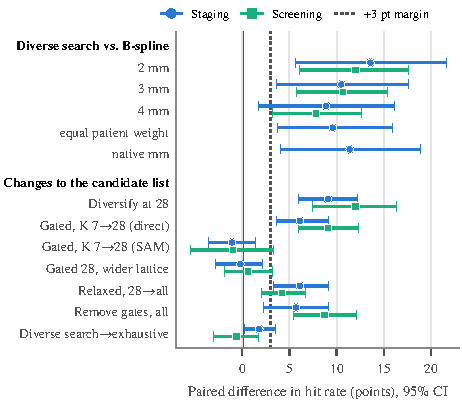
\includegraphics[width=\linewidth]{figures/paired_forest.pdf}
\caption{\textbf{Paired differences with 95\% patient-cluster intervals.} Top: \ours minus B-spline at three tolerances and in two robustness analyses (staging only). Bottom: changes to the candidate list at 3\,mm (Tab.~\ref{tab:contrasts}). The dashed line is the 3-point margin fixed before inference; an interval entirely to the right of zero is a significant gain.}
\label{fig:forest}
\end{figure}

\begin{figure*}[!t]
\centering
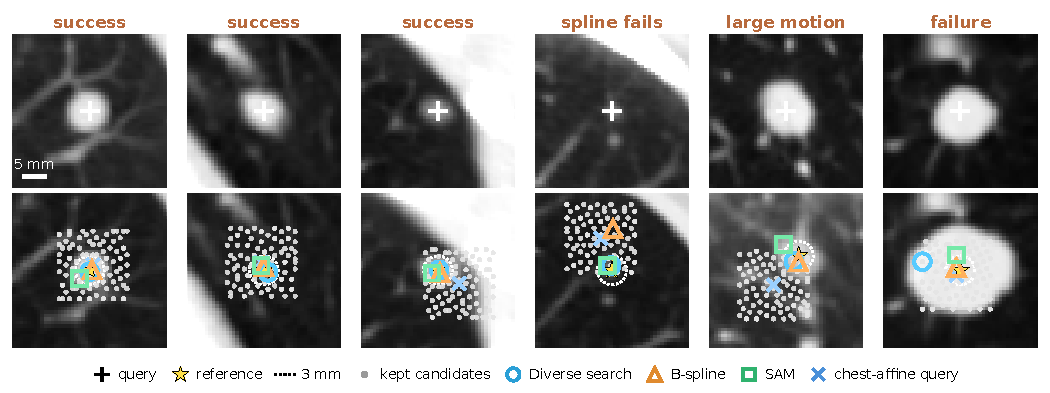
\includegraphics[width=\linewidth]{figures/qualitative.pdf}
\caption{Qualitative examples from the staging cohort. The columns are three successes, one spline failure, one large-motion case, and one failure of Diverse search. Top: current CT with the query ($+$). Bottom: earlier CT with the reference (star) and a 3 mm tolerance (dotted), the kept candidates (small dots), and the points selected by Diverse search (circle), the B-spline (triangle), and SAM (square). The cross is where the chest affine places the query.}
\label{fig:qualitative}

\end{figure*}

\subsection{Sensitivity to the query}
\label{sec:query}
Because the query is simulated by jittering the annotated mark, part of the gain could come from lesions whose query starts far away.
Figure~\ref{fig:bands} splits lesions by the distance between the query $p$ and the annotated current mark.
Among lesions whose query is within 1.5\,mm, \ours hits 238 of 322 staging lesions versus 205 for the spline ($+10.2$ points [2.1, 18.4]) and 178 versus 157 of 194 screening lesions ($+10.8$ [5.8, 16.0]).
This well-localized band contributes 33 of the 46 net staging gains and 21 of the 33 screening gains.
The smaller bands have wide intervals and are descriptive.

We also reran the screening cohort with the exact annotated mark as the query.
The spline improves from 211 to 239 hits, while \ours is essentially unchanged (244 to 243).
With a perfect query the screening advantage therefore shrinks from 33 to 4 hits, so a large part of it reflects robustness to an imprecise query (supplement, Tab.~S7).
We return to this in Sec.~\ref{sec:discussion}.

\begin{figure}[!t]
\centering
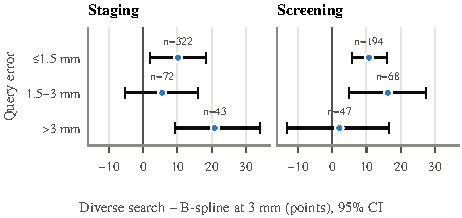
\includegraphics[width=\linewidth]{figures/query_bands.pdf}
\caption{\textbf{Gain by query error.} Paired 3\,mm difference between \ours and the B-spline within bands of query error (distance between $p$ and the annotated current mark), with 95\% patient-cluster intervals; $n$ is the number of lesions per band. Three unsupported staging queries are excluded here but counted in Tab.~\ref{tab:main}.}
\label{fig:bands}
\end{figure}

\subsection{Diversification makes better use of a fixed budget}
\label{sec:diversity}
At a budget of 28, the fit-ordered list spends several slots on the same neighborhood.
Enforcing 2.1\,mm separation, with the same order, grid and scorer, raises reach from 221 to 274 staging lesions and from 189 to 242 screening lesions, and raises hits from 205 to 245 ($+9.1$ points [6.0, 12.2]) and from 175 to 212 ($+12.0$ points [7.5, 16.4]) (Tab.~\ref{tab:contrasts}).
Figure~\ref{fig:attribution} applies Eq.~\ref{eq:decomp}.
Diversification makes 54 staging and 56 screening lesions newly reachable, and the scorer selects 45 and 41 of them, while choices on lesions reachable by both lists lose a net four hits in each cohort.
The gain is therefore a gain in coverage, not in selection.
The same holds with relaxed gates, where diversification at 28 adds 7.5 [4.7, 10.7] and 9.4 [5.3, 13.4] points.

\begin{figure}[!t]
\centering
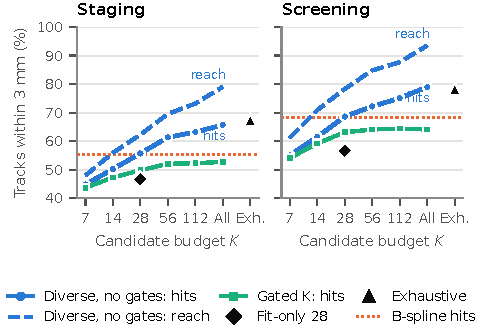
\includegraphics[width=\linewidth]{figures/budget_reach.pdf}
\caption{\textbf{Reach and hits versus candidate budget} at fixed wide extent and image support. Dashed: share of lesions with any candidate within 3\,mm (reach). Solid: share whose selected point is within 3\,mm (hits). At $K{=}28$ the diversified list (blue) beats the fit-only list (diamond) by 9.1 and 12.0 points; hard gates (green) limit the benefit of a larger budget. Exh.: all 4,851 positions.}
\label{fig:budget}
\end{figure}

\begin{table}[!t]
\centering
\footnotesize
\setlength{\tabcolsep}{2.2pt}
\begin{tabular}{@{}llccc@{}}
\toprule
& Change & Reach & Hits & $+$/$-$ \\
\midrule
\multirow{7}{*}{\rotatebox{90}{Staging}}
& Diversify at 28 & 221$\to$274 & 205$\to$245 & 51/11 \\
& Strict 7$\to$28, direct & 202$\to$241 & 192$\to$219 & 34/7 \\
& Strict 7$\to$28, SAM & 202$\to$241 & 144$\to$139 & 17/22 \\
& Wider lattice at 28 & 239$\to$241 & 220$\to$219 & 15/16 \\
& Relaxed 28$\to$all & 264$\to$300 & 237$\to$264 & 33/6 \\
& Remove gates, all & 300$\to$348 & 264$\to$289 & 30/5 \\
& Diverse$\to$exhaustive & 348$\to$351 & 289$\to$297 & 12/4 \\
\midrule
\multirow{7}{*}{\rotatebox{90}{Screening}}
& Diversify at 28 & 189$\to$242 & 175$\to$212 & 44/7 \\
& Strict 7$\to$28, direct & 185$\to$220 & 167$\to$195 & 28/0 \\
& Strict 7$\to$28, SAM & 185$\to$220 & 121$\to$118 & 23/26 \\
& Wider lattice at 28 & 220$\to$220 & 193$\to$195 & 9/7 \\
& Relaxed 28$\to$all & 235$\to$257 & 204$\to$217 & 14/1 \\
& Remove gates, all & 257$\to$289 & 217$\to$244 & 29/2 \\
& Diverse$\to$exhaustive & 289$\to$290 & 244$\to$242 & 6/8 \\
\bottomrule
\end{tabular}
\caption{Paired changes to the candidate list at 3\,mm on all 440 staging and 309 screening lesions. $+$/$-$ counts lesions that become hits / stop being hits. Differences in points with 95\% intervals are plotted in Fig.~\ref{fig:forest}.}
\label{tab:contrasts}
\end{table}


Figure~\ref{fig:budget} follows reach and hits as the budget grows.
The complete diversified list reaches 348 of the 351 lesions reachable on the full lattice in staging and 289 of 290 in screening, while scoring about one-thirteenth of the positions.
The coverage bound (Eq.~\ref{eq:coverage}) also predicts a cost: one kept point represents a cluster of nearby translations, which matters more at tight tolerances.
Indeed, exhaustive scoring adds 18 staging hits over \ours at 2\,mm but only five at 4\,mm.

\subsection{Additional reach pays off only with a capable scorer}
\label{sec:scorer}
Raising the strict cap from 7 to 28 increases direct hits from 192 to 219 on staging ($+6.1$ points [3.6, 9.1]) and from 167 to 195 on screening ($+9.1$ points [6.0, 12.3]), both above the prespecified margin.
Widening the lattice at fixed support and cap 28 does not help (intervals span zero), so the number and placement of kept candidates, not the lattice extent, drive the gain.
On the identical expanded lists, the direct scorer selects 33 of the 39 newly reachable staging lesions, whereas SAM selects only 10 and loses 15 hits on the 202 shared lesions (Fig.~\ref{fig:attribution}).
The cap effect favors the direct scorer over SAM by 7.3 points [4.4, 10.4] on staging and 10.0 [5.4, 14.8] on screening.
A larger candidate budget is useful only to a scorer that can exploit it.

\begin{figure}[!t]
\centering
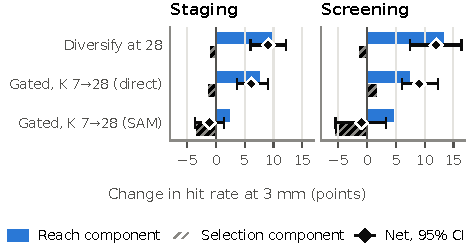
\includegraphics[width=\linewidth]{figures/reach_selection.pdf}
\caption{\textbf{Where additional hits come from} (Eq.~\ref{eq:decomp}), in points. Blue: reach term (hits on newly reachable lesions minus hits lost with reach). Hatched: selection term (change on lesions reachable by both lists). Black: net change with its 95\% interval. Diversification and a larger cap gain through reach with the direct scorer; SAM, given identical candidates, loses more on shared lesions than it gains.}
\label{fig:attribution}
\end{figure}

Hard gates also discard usable candidates.
With relaxed gates, replacing cap 28 by the complete list raises hits from 237 to 264 (staging) and from 204 to 217 (screening).
Removing the remaining gates adds 48 and 32 reachable lesions and 25 and 27 hits.
Since anatomical fit still enters Eq.~\ref{eq:direct}, this supports using fit as a soft preference rather than a hard filter.

\subsection{Compute}
\label{sec:latency}
On prepared staging crops, the median local time is 0.194\,s for \ours versus 3.617\,s for the spline (18.6$\times$), and 0.185 versus 3.866\,s on screening (20.9$\times$); p90 times are 0.458 versus 4.707\,s and 0.190 versus 4.693\,s.
Figure~\ref{fig:speed} places every fixed budget on one accuracy--latency plot.
The diversified 28-point list costs 22\,ms more than the fit-only list for 40 additional staging hits.
A cap of 112 gives 278 staging hits at 0.142\,s, saving a median 50\,ms [45, 53] per query relative to the complete list, an intermediate operating point.
With native scans, chest alignment dominates: one query per screening pair takes 29.36\,s for \ours versus 32.87\,s for the spline, and two queries sharing the alignment take 14.88 versus 19.38\,s per query.
The local speedup therefore matters most when the alignment is shared across many lesions.

\begin{figure}[!t]
\centering
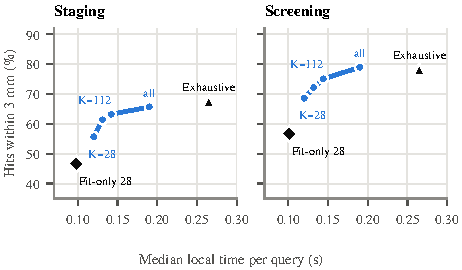
\includegraphics[width=\linewidth]{figures/accuracy_latency.pdf}
\caption{\textbf{Accuracy versus prepared-crop latency.} Diverse search at caps 28, 56, 112 and the complete list, the fit-only list and exhaustive scoring come from a three-repeat randomized replay on matched workloads of 24 staging and 32 screening queries; the spline point is from the matched prepared-crop comparison. Hit rates use the full cohorts.}
\label{fig:speed}
\end{figure}

\section{Discussion and limitations}
\label{sec:discussion}
For a point query in an aligned scan pair, anatomy can order plausible translations cheaply, while a lesion scorer chooses among their positions.
Our equal-budget comparisons show that changing only \emph{where} the candidates lie, not how many are scored, improves matching in both cohorts.
Separating reach from selection explains the gain: diversification creates opportunities, and the scorer determines how many are realized.
The same accounting shows that a general anatomical embedding does not benefit from extra candidates that a lesion-specific scorer exploits.

\paragraph{Limitations.}
The task assumes an approximate current location and a known persistent lesion; clinical incident status and wrong-lesion associations require separate adjudication.
The query is simulated by jittering the annotated mark, and with the exact mark the screening advantage over the spline shrinks from 33 to 4 hits (Sec.~\ref{sec:query}); evaluating with queries from a real detector or real clicks is needed.
% TODO(group): agree on this wording.
A failed chest alignment can leave the lesion outside the local crop: in two staging pairs, 28 references lie more than 100\,mm outside the crop and every method errs by more than 200\,mm; these lesions remain in the denominators.
The screening cohort is retrospective, whereas the staging cohort is the independent test.
End-to-end time on native scans is dominated by the shared chest alignment.
Finally, we did not compare with learned registration models, which could provide a stronger continuous baseline.

\section{Conclusion}
\label{sec:conclusion}
We studied how to choose the candidate locations that a lesion scorer sees when matching a lung lesion across CT visits.
Ranking candidates by anatomical fit and keeping only those at least 2.1\,mm apart spreads a fixed budget over more distinct locations, and the complete list covers the full lattice to within that distance at about one-thirteenth of the cost.
On an independent staging cohort and a screening cohort, this simple rule outperforms a lesion-inclusive B-spline by about 10 points at 3\,mm while running about 19 times faster on the local step.
Our reach/selection decomposition shows that the gain comes from coverage, and that it pays off only with a scorer able to use the extra candidates.
Future work includes real query sources, scorers trained to exploit diverse candidate lists, and other anatomies where several nearby locations are plausible.


\label{sec:main-end}
\section*{LLM Usage Statement}
OpenAI Codex assisted with study design, literature and data screening, code, experiment execution, analysis, figures and tables, manuscript drafting and editing, and source and layout checks. The numerical results are computed from the specified inputs using the recorded analysis. The authors are responsible for verification and for the submitted work.

{\small
\bibliographystyle{ieeenat_fullname}
\bibliography{refs}
}
\end{document}
